% Options for packages loaded elsewhere
%DIF LATEXDIFF DIFFERENCE FILE
%DIF DEL C:\Users\erobin17\Documents\publications\2022-sdss-you-draw-it-manuscript\original-2022-sdss-you-draw-it-manuscript.tex   Fri Oct 28 09:54:19 2022
%DIF ADD C:\Users\erobin17\Documents\publications\2022-sdss-you-draw-it-manuscript\2022-sdss-you-draw-it-manuscript.tex            Mon Nov 14 07:20:37 2022
\PassOptionsToPackage{unicode}{hyperref}
\PassOptionsToPackage{hyphens}{url}
\PassOptionsToPackage{dvipsnames,svgnames,x11names}{xcolor}
%
\documentclass[
]{jds}

\usepackage{amsmath,amssymb}
\usepackage{lmodern}
\usepackage{iftex}
\ifPDFTeX
  \usepackage[T1]{fontenc}
  \usepackage[utf8]{inputenc}
  \usepackage{textcomp} % provide euro and other symbols
\else % if luatex or xetex
  \usepackage{unicode-math}
  \defaultfontfeatures{Scale=MatchLowercase}
  \defaultfontfeatures[\rmfamily]{Ligatures=TeX,Scale=1}
\fi
% Use upquote if available, for straight quotes in verbatim environments
\IfFileExists{upquote.sty}{\usepackage{upquote}}{}
\IfFileExists{microtype.sty}{% use microtype if available
  \usepackage[]{microtype}
  \UseMicrotypeSet[protrusion]{basicmath} % disable protrusion for tt fonts
}{}
\makeatletter
\@ifundefined{KOMAClassName}{% if non-KOMA class
  \IfFileExists{parskip.sty}{%
    \usepackage{parskip}
  }{% else
    \setlength{\parindent}{0pt}
    \setlength{\parskip}{6pt plus 2pt minus 1pt}}
}{% if KOMA class
  \KOMAoptions{parskip=half}}
\makeatother
\usepackage{xcolor}
\setlength{\emergencystretch}{3em} % prevent overfull lines
\setcounter{secnumdepth}{-\maxdimen} % remove section numbering
% Make \paragraph and \subparagraph free-standing
\ifx\paragraph\undefined\else
  \let\oldparagraph\paragraph
  \renewcommand{\paragraph}[1]{\oldparagraph{#1}\mbox{}}
\fi
\ifx\subparagraph\undefined\else
  \let\oldsubparagraph\subparagraph
  \renewcommand{\subparagraph}[1]{\oldsubparagraph{#1}\mbox{}}
\fi


\providecommand{\tightlist}{%
  \setlength{\itemsep}{0pt}\setlength{\parskip}{0pt}}\usepackage{longtable,booktabs,array}
\usepackage{calc} % for calculating minipage widths
% Correct order of tables after \paragraph or \subparagraph
\usepackage{etoolbox}
\makeatletter
\patchcmd\longtable{\par}{\if@noskipsec\mbox{}\fi\par}{}{}
\makeatother
% Allow footnotes in longtable head/foot
\IfFileExists{footnotehyper.sty}{\usepackage{footnotehyper}}{\usepackage{footnote}}
\makesavenoteenv{longtable}
\usepackage{graphicx}
\makeatletter
\def\maxwidth{\ifdim\Gin@nat@width>\linewidth\linewidth\else\Gin@nat@width\fi}
\def\maxheight{\ifdim\Gin@nat@height>\textheight\textheight\else\Gin@nat@height\fi}
\makeatother
% Scale images if necessary, so that they will not overflow the page
% margins by default, and it is still possible to overwrite the defaults
% using explicit options in \includegraphics[width, height, ...]{}
\setkeys{Gin}{width=\maxwidth,height=\maxheight,keepaspectratio}
% Set default figure placement to htbp
\makeatletter
\def\fps@figure{htbp}
\makeatother
\newlength{\cslhangindent}
\setlength{\cslhangindent}{1.5em}
\newlength{\csllabelwidth}
\setlength{\csllabelwidth}{3em}
\newlength{\cslentryspacingunit} % times entry-spacing
\setlength{\cslentryspacingunit}{\parskip}
\newenvironment{CSLReferences}[2] % #1 hanging-ident, #2 entry spacing
 {% don't indent paragraphs
  \setlength{\parindent}{0pt}
  % turn on hanging indent if param 1 is 1
  \ifodd #1
  \let\oldpar\par
  \def\par{\hangindent=\cslhangindent\oldpar}
  \fi
  % set entry spacing
  \setlength{\parskip}{#2\cslentryspacingunit}
 }%
 {}
\usepackage{calc}
\newcommand{\CSLBlock}[1]{#1\hfill\break}
\newcommand{\CSLLeftMargin}[1]{\parbox[t]{\csllabelwidth}{#1}}
\newcommand{\CSLRightInline}[1]{\parbox[t]{\linewidth - \csllabelwidth}{#1}\break}
\newcommand{\CSLIndent}[1]{\hspace{\cslhangindent}#1}

\usepackage[dvipsnames]{xcolor} % colors
\newcommand{\ear}[1]{{\textcolor{blue}{#1}}}
\newcommand{\svp}[1]{{\textcolor{RedOrange}{#1}}}
\newcommand{\rh}[1]{{\textcolor{Green}{#1}}}
\author[1]{Emily A. Robinson\thanks{Corresponding author. Email: erobin17@calpoly.edu}}
\author[2]{Reka Howard\footnote{Email: rekahoward@unl.edu}}
\author[2]{Susan VanderPlas\footnote{Email: susan.vanderplas@unl.edu}}
\affil[1]{Department of Statistics, CalPoly-San Luis Obispo}
\affil[2]{Department of Statistics, University of Nebraska-Lincoln}
\makeatletter
\makeatother
\makeatletter
\makeatother
\makeatletter
\@ifpackageloaded{caption}{}{\usepackage{caption}}
\AtBeginDocument{%
\ifdefined\contentsname
  \renewcommand*\contentsname{Table of contents}
\else
  \newcommand\contentsname{Table of contents}
\fi
\ifdefined\listfigurename
  \renewcommand*\listfigurename{List of Figures}
\else
  \newcommand\listfigurename{List of Figures}
\fi
\ifdefined\listtablename
  \renewcommand*\listtablename{List of Tables}
\else
  \newcommand\listtablename{List of Tables}
\fi
\ifdefined\figurename
  \renewcommand*\figurename{Figure}
\else
  \newcommand\figurename{Figure}
\fi
\ifdefined\tablename
  \renewcommand*\tablename{Table}
\else
  \newcommand\tablename{Table}
\fi
}
\@ifpackageloaded{float}{}{\usepackage{float}}
\floatstyle{ruled}
\@ifundefined{c@chapter}{\newfloat{codelisting}{h}{lop}}{\newfloat{codelisting}{h}{lop}[chapter]}
\floatname{codelisting}{Listing}
\newcommand*\listoflistings{\listof{codelisting}{List of Listings}}
\makeatother
\makeatletter
\@ifpackageloaded{caption}{}{\usepackage{caption}}
\@ifpackageloaded{subcaption}{}{\usepackage{subcaption}}
\makeatother
\makeatletter
\@ifpackageloaded{tcolorbox}{}{\usepackage[many]{tcolorbox}}
\makeatother
\makeatletter
\@ifundefined{shadecolor}{\definecolor{shadecolor}{rgb}{.97, .97, .97}}
\makeatother
\makeatletter
\makeatother
\ifLuaTeX
  \usepackage{selnolig}  % disable illegal ligatures
\fi
\IfFileExists{bookmark.sty}{\usepackage{bookmark}}{\usepackage{hyperref}}
\IfFileExists{xurl.sty}{\usepackage{xurl}}{} % add URL line breaks if available
\urlstyle{same} % disable monospaced font for URLs
\hypersetup{
  pdftitle={`You Draw It': Implementation of visually fitted trends with r2d3},
  pdfkeywords={graphics, user interaction, regression},
  colorlinks=true,
  linkcolor={blue},
  filecolor={Maroon},
  citecolor={Blue},
  urlcolor={Blue},
  pdfcreator={LaTeX via pandoc}}

\title{`You Draw It': Implementation of visually fitted trends with
\texttt{r2d3}}
% \author{}
%DIF < \date{}
%DIF -------
% \date{} %DIF > 
%DIF PREAMBLE EXTENSION ADDED BY LATEXDIFF
%DIF UNDERLINE PREAMBLE %DIF PREAMBLE
\RequirePackage[normalem]{ulem} %DIF PREAMBLE
\RequirePackage{color}\definecolor{RED}{rgb}{1,0,0}\definecolor{BLUE}{rgb}{0,0,1} %DIF PREAMBLE
\providecommand{\DIFaddtex}[1]{{\protect\color{blue}\uwave{#1}}} %DIF PREAMBLE
\providecommand{\DIFdeltex}[1]{{\protect\color{red}\sout{#1}}}                      %DIF PREAMBLE
%DIF SAFE PREAMBLE %DIF PREAMBLE
\providecommand{\DIFaddbegin}{} %DIF PREAMBLE
\providecommand{\DIFaddend}{} %DIF PREAMBLE
\providecommand{\DIFdelbegin}{} %DIF PREAMBLE
\providecommand{\DIFdelend}{} %DIF PREAMBLE
\providecommand{\DIFmodbegin}{} %DIF PREAMBLE
\providecommand{\DIFmodend}{} %DIF PREAMBLE
%DIF FLOATSAFE PREAMBLE %DIF PREAMBLE
\providecommand{\DIFaddFL}[1]{\DIFadd{#1}} %DIF PREAMBLE
\providecommand{\DIFdelFL}[1]{\DIFdel{#1}} %DIF PREAMBLE
\providecommand{\DIFaddbeginFL}{} %DIF PREAMBLE
\providecommand{\DIFaddendFL}{} %DIF PREAMBLE
\providecommand{\DIFdelbeginFL}{} %DIF PREAMBLE
\providecommand{\DIFdelendFL}{} %DIF PREAMBLE
%DIF HYPERREF PREAMBLE %DIF PREAMBLE
\providecommand{\DIFadd}[1]{\texorpdfstring{\DIFaddtex{#1}}{#1}} %DIF PREAMBLE
\providecommand{\DIFdel}[1]{\texorpdfstring{\DIFdeltex{#1}}{}} %DIF PREAMBLE
\newcommand{\DIFscaledelfig}{0.5}
%DIF HIGHLIGHTGRAPHICS PREAMBLE %DIF PREAMBLE
\RequirePackage{settobox} %DIF PREAMBLE
\RequirePackage{letltxmacro} %DIF PREAMBLE
\newsavebox{\DIFdelgraphicsbox} %DIF PREAMBLE
\newlength{\DIFdelgraphicswidth} %DIF PREAMBLE
\newlength{\DIFdelgraphicsheight} %DIF PREAMBLE
% store original definition of \includegraphics %DIF PREAMBLE
\LetLtxMacro{\DIFOincludegraphics}{\includegraphics} %DIF PREAMBLE
\newcommand{\DIFaddincludegraphics}[2][]{{\color{blue}\fbox{\DIFOincludegraphics[#1]{#2}}}} %DIF PREAMBLE
\newcommand{\DIFdelincludegraphics}[2][]{% %DIF PREAMBLE
\sbox{\DIFdelgraphicsbox}{\DIFOincludegraphics[#1]{#2}}% %DIF PREAMBLE
\settoboxwidth{\DIFdelgraphicswidth}{\DIFdelgraphicsbox} %DIF PREAMBLE
\settoboxtotalheight{\DIFdelgraphicsheight}{\DIFdelgraphicsbox} %DIF PREAMBLE
\scalebox{\DIFscaledelfig}{% %DIF PREAMBLE
\parbox[b]{\DIFdelgraphicswidth}{\usebox{\DIFdelgraphicsbox}\\[-\baselineskip] \rule{\DIFdelgraphicswidth}{0em}}\llap{\resizebox{\DIFdelgraphicswidth}{\DIFdelgraphicsheight}{% %DIF PREAMBLE
\setlength{\unitlength}{\DIFdelgraphicswidth}% %DIF PREAMBLE
\begin{picture}(1,1)% %DIF PREAMBLE
\thicklines\linethickness{2pt} %DIF PREAMBLE
{\color[rgb]{1,0,0}\put(0,0){\framebox(1,1){}}}% %DIF PREAMBLE
{\color[rgb]{1,0,0}\put(0,0){\line( 1,1){1}}}% %DIF PREAMBLE
{\color[rgb]{1,0,0}\put(0,1){\line(1,-1){1}}}% %DIF PREAMBLE
\end{picture}% %DIF PREAMBLE
}\hspace*{3pt}}} %DIF PREAMBLE
} %DIF PREAMBLE
\LetLtxMacro{\DIFOaddbegin}{\DIFaddbegin} %DIF PREAMBLE
\LetLtxMacro{\DIFOaddend}{\DIFaddend} %DIF PREAMBLE
\LetLtxMacro{\DIFOdelbegin}{\DIFdelbegin} %DIF PREAMBLE
\LetLtxMacro{\DIFOdelend}{\DIFdelend} %DIF PREAMBLE
\DeclareRobustCommand{\DIFaddbegin}{\DIFOaddbegin \let\includegraphics\DIFaddincludegraphics} %DIF PREAMBLE
\DeclareRobustCommand{\DIFaddend}{\DIFOaddend \let\includegraphics\DIFOincludegraphics} %DIF PREAMBLE
\DeclareRobustCommand{\DIFdelbegin}{\DIFOdelbegin \let\includegraphics\DIFdelincludegraphics} %DIF PREAMBLE
\DeclareRobustCommand{\DIFdelend}{\DIFOaddend \let\includegraphics\DIFOincludegraphics} %DIF PREAMBLE
\LetLtxMacro{\DIFOaddbeginFL}{\DIFaddbeginFL} %DIF PREAMBLE
\LetLtxMacro{\DIFOaddendFL}{\DIFaddendFL} %DIF PREAMBLE
\LetLtxMacro{\DIFOdelbeginFL}{\DIFdelbeginFL} %DIF PREAMBLE
\LetLtxMacro{\DIFOdelendFL}{\DIFdelendFL} %DIF PREAMBLE
\DeclareRobustCommand{\DIFaddbeginFL}{\DIFOaddbeginFL \let\includegraphics\DIFaddincludegraphics} %DIF PREAMBLE
\DeclareRobustCommand{\DIFaddendFL}{\DIFOaddendFL \let\includegraphics\DIFOincludegraphics} %DIF PREAMBLE
\DeclareRobustCommand{\DIFdelbeginFL}{\DIFOdelbeginFL \let\includegraphics\DIFdelincludegraphics} %DIF PREAMBLE
\DeclareRobustCommand{\DIFdelendFL}{\DIFOaddendFL \let\includegraphics\DIFOincludegraphics} %DIF PREAMBLE
%DIF COLORLISTINGS PREAMBLE %DIF PREAMBLE
\RequirePackage{listings} %DIF PREAMBLE
\RequirePackage{color} %DIF PREAMBLE
\lstdefinelanguage{DIFcode}{ %DIF PREAMBLE
%DIF DIFCODE_UNDERLINE %DIF PREAMBLE
  moredelim=[il][\color{red}\sout]{\%DIF\ <\ }, %DIF PREAMBLE
  moredelim=[il][\color{blue}\uwave]{\%DIF\ >\ } %DIF PREAMBLE
} %DIF PREAMBLE
\lstdefinestyle{DIFverbatimstyle}{ %DIF PREAMBLE
	language=DIFcode, %DIF PREAMBLE
	basicstyle=\ttfamily, %DIF PREAMBLE
	columns=fullflexible, %DIF PREAMBLE
	keepspaces=true %DIF PREAMBLE
} %DIF PREAMBLE
\lstnewenvironment{DIFverbatim}{\lstset{style=DIFverbatimstyle}}{} %DIF PREAMBLE
\lstnewenvironment{DIFverbatim*}{\lstset{style=DIFverbatimstyle,showspaces=true}}{} %DIF PREAMBLE
%DIF END PREAMBLE EXTENSION ADDED BY LATEXDIFF

\begin{document}
\maketitle
\begin{abstract}
How do statistical regression results compare to intuitive, visually
fitted results? Fitting lines by eye through a set of points has been
explored since the 20th century. Common methods of fitting trends by eye
involve maneuvering a string, black thread, or ruler until the fit is
suitable, then drawing the line through the set of points. In 2015, the
New York Times introduced an interactive feature, called `You Draw It,'
where readers are asked to input their own assumptions about various
metrics and compare how these assumptions relate to reality. This
research is intended to implement `You Draw It', adapted from the New
York Times, as a way to measure the patterns we see in data. In this
paper, we describe the adaptation of an old tool for graphical testing
and evaluation, eye-fitting, for use in modern web-applications suitable
for testing statistical graphics. We present an empirical evaluation of
this testing method for linear regression, and briefly discuss an
extension of this method to non-linear applications.
\end{abstract}
\ifdefined\Shaded\DIFdelbegin %DIFDELCMD < \renewenvironment{Shaded}{\begin{tcolorbox}[borderline west={3pt}{0pt}{shadecolor}, frame hidden, enhanced, breakable, sharp corners, interior hidden, boxrule=0pt]}{\end{tcolorbox}}%%%
\DIFdelend \DIFaddbegin \renewenvironment{Shaded}{\begin{tcolorbox}[boxrule=0pt, sharp corners, borderline west={3pt}{0pt}{shadecolor}, breakable, enhanced, frame hidden, interior hidden]}{\end{tcolorbox}}\DIFaddend \fi

\hypertarget{introduction}{%
\section{Introduction}\label{introduction}}

We all use statistical graphics, but how do we know that the graphics we
use are communicating effectively? Through experimentation, graphical
testing methods allow researchers to conduct studies designed to
understand how we perceive graphics and perform graphical tasks such as
differentiation, prediction, estimation, and extrapolation. Each of
these levels of interaction with a graph require a different method of
engagement with and use of the information presented in a chart. In this
paper, we describe the adaptation of an old tool for graphical testing
and evaluation, eye-fitting, for use in modern web-applications suitable
for testing statistical graphics. We present an empirical evaluation of
this testing method for linear regression, and briefly discuss an
extension of this method to non-linear applications.

One of the most common charts created is a scatterplot of points over
time; these charts show up regularly in news articles and in scientific
publications alike. These charts rely on our ability to identify and
detect trends in data. Our visual system is naturally built to look for
structure and identify patterns, including patterns and trends over
time; many times we do not even notice this process happening
subconsciously. As shown in Figure~\ref{fig-gas-prices}, a viewer
engaging with a plot of weekly average gas prices over time may perform
several cognitive operations. First, they scan the plot and assesses
points to determine if there are any outliers or otherwise remarkable
points. Then, they may fit a rough mental smooth/trend line to the
points to summarize the useful information and remove variability.
Finally, an interested and engaged viewer may pull in additional
contextual information from long-term memory, seeking to explain
variation in the mental `trend' with supplemental information, such as
COVID lock downs which reduced gasoline demand and the beginning of the
war in Ukraine, which wreaked havoc on the supply and demand for global
energy sources.

\begin{figure}

{\centering \includegraphics{./images/fig-gas-prices-1.pdf}

}

\caption{\label{fig-gas-prices}\DIFdelbeginFL \DIFdelFL{Weekly }\DIFdelendFL \DIFaddbeginFL \DIFaddFL{Demonstration of a viewer's engagement
with a scatterplot showing the weekly }\DIFaddendFL average gas prices in the United
States, \DIFaddbeginFL \DIFaddFL{from }\DIFaddendFL 2019-June 2022. \DIFdelbeginFL \DIFdelFL{Additional mental operations a viewer }\DIFdelendFL \DIFaddbeginFL \DIFaddFL{The veiwer }\DIFaddendFL might perform \DIFdelbeginFL \DIFdelFL{while looking at }\DIFdelendFL \DIFaddbeginFL \DIFaddFL{several cognitive
operations such as assessing points to determine outliers, fitting a
rough mental smooth/trend line (overlaying solid gray line), and using
additional contextual information from long term memory to explain }\DIFaddendFL the
\DIFdelbeginFL \DIFdelFL{plot are }\DIFdelendFL \DIFaddbeginFL \DIFaddFL{variation (shaded rectangular gray regions }\DIFaddendFL annotated in \DIFdelbeginFL \DIFdelFL{grey }\DIFdelendFL \DIFaddbeginFL \DIFaddFL{black text) }\DIFaddendFL (US
Energy Information Administration 2022).}

\end{figure}

Initial studies in the 20th century explored the use of fitting lines by
eye through a set of points (Finney 1951; Mosteller et al. 1981; \DIFaddbegin \DIFadd{A. R.
}\DIFaddend Unwin and Wills 1988). Common methods of fitting trends by eye involved
maneuvering a string, black thread, or ruler until the fit was suitable,
then drawing the line through the set of points. Results from these
early studies provided groundwork for visually judging slopes and
selecting accurate starting values for common iterative calculations.
Recently, Ciccione and Dehaene (2021) conducted a comprehensive set of
studies investigating human ability to detect trends in graphical
representations from a psychophysical approach. This set of studies
asked participants to judge trends, estimate slopes, and conduct
extrapolation by using a track-pad to adjust the tilt of a line on the
screen. Results indicated the slopes participants reported were always
in excess of the ideal slopes, both in the positive and in the negative
direction, and those biases increased with noise and with number of
points. This supported the results found in Mosteller et al. (1981) and
suggested that participants might use Deming regression (Deming 1943),
which minimizes the Euclidean distance of points from the line, when
fitting a line to a noisy scatterplot.

While psychologists and statisticians have been using eye-fitting
techniques to assess our innate perceptual statistical modeling
abilities, news organizations have used similar techniques in order to
draw readers in and demonstrate the difference between readers'
assumptions and reality. In 2015, the New York Times (NYT) introduced an
interactive feature, called `You Draw It' (Aisch, Cox, and Quealy 2015),
where readers input their own assumptions about various metrics of news
interest and compare these assumptions to reality. The NYT team used
Data Driven Documents (D3), a JavaScript library that allows readers to
interact with a chart directly by drawing a line on their computer
screen with a mouse. Despite the somewhat different purpose behind this
feature, the D3 driven method used by the NYT is wonderfully intuitive,
and does not require the assumption of linearity, making it much more
adaptable to testing how viewers perceive and predict when presented
with non-linear data.

We set out to implement `You Draw It', adapted from the NYT feature, as
a way to experimentally assess the patterns we see in data. Here, we
provide technical details of the software development, utilizing
interactive graphics in R (R Core Team 2022). We then share results from
our study which validates `You Draw It' as a method for graphical
testing on linear trends and apply an appropriate data analysis method
to the participant data. We also briefly demonstrate the use of the `You
Draw It' method and analysis on non-linear data.

\hypertarget{development}{%
\section{Development}\label{development}}

\hypertarget{you-draw-it-v0}{%
\subsection{`You Draw It' v0}\label{you-draw-it-v0}}

The NYT uses D3, Data Driven Documents (Bostock, Ogievetsky, and Heer
2011), to create many of the interactive data graphics that users rely
on, from the famous ``election needle'' in 2016 to their COVID
dashboards. Naturally, this same framework was used to create the `You
Draw It' feature. The NYT code used to create the initial D3 plot and
`You Draw It' interactive feature includes multiple working parts.
First, the relationship between coordinate mappings and pixels sets up
the chart and the initial data is plotted. Next, the \texttt{d3.drag}
function adds user interactivity and observes the movement of the user's
mouse. Additionally, the \texttt{forEach} loop finds the closest point
in the coordinate system to the user's mouse. Finally, the code detects
if all points are filled by the user and updates the status of the task.

When working with a new programming language, setting up a new
development environment can be challenging. As R users, we found the
software overhead required to develop straight JavaScript code to be
intimidating (Wattenberger 2019), but luckily, the R community
anticipated this barrier. In the next section, we will see how the
\texttt{r2d3} package (Strayer, Luraschi, and Allaire 2020) in R can be
used to render the JavaScript code and display D3 visuals in familiar R
HTML formats such as Rmarkdown and Shiny.

\hypertarget{generating-d3-plots-in-r}{%
\subsection{Generating D3 Plots in R}\label{generating-d3-plots-in-r}}

We leveraged the \texttt{r2d3} package to take data randomly generated
in R and create a D3 plot that could be modified with the `You Draw It'
script. This step allowed us to more easily connect the data generation
process with the resulting D3 code without having to generate new code
manually each time we re-generated the data. While not strictly
necessary for the validation test of the `You Draw It' method compared
to past linear regression methods presented in this paper, this
abstraction makes it much easier to test arbitrary or model-generated
data which is unique to each participant.

We conducted all data simulation and processing in R and output two data
sets - \emph{point data} and \emph{line data} - containing \((x, y)\)
coordinates corresponding to either a simulated point or fitted value
predicted by a statistical model respectively. Then, the \texttt{r2d3}
package converts the data sets in R to JavaScript Object Notation (JSON)
to be interpreted by JavaScript code included with the \texttt{r2d3}
package. Parameters for aesthetic design choices are defined in a list
of options in the \texttt{r2d3} function call; \texttt{r2d3} passes
these to the generated JavaScript code. For instance, we can specify the
buffer space allowed for the \(x\) and \(y\) axes to avoid users
anchoring their lines to the axes limits.

\hypertarget{adding-you-draw-it-functionality}{%
\subsection{Adding `You Draw It'
Functionality}\label{adding-you-draw-it-functionality}}

In order to make use of the original `You Draw It' code for perceptual
experiments, we first needed to accommodate an additional layer. The
original NYT features asked participants to draw on a blank coordinate
grid, as shown in Figure~\ref{fig-nyt-screenshot}.

\begin{figure}

{\centering \includegraphics{images/NYT-You-Draw-It-Screenshot.png}

}

\caption{\label{fig-nyt-screenshot}Screenshot of the
\href{https://www.nytimes.com/interactive/2015/05/28/upshot/you-draw-it-how-family-income-affects-childrens-college-chances.html}{You
Draw It application} originally developed by the New York Times.}

\end{figure}

When testing perception of graphics, however, we want to pre-populate
the chart with additional information - points, and in some cases,
portions of a trend line. This requires that we modify the original
JavaScript source code to accommodate these additional elements, which
we generate using \texttt{r2d3}, as described above.

As previously discussed, we modified \texttt{r2d3} code to draw the
initial plot and data. Drag events in \texttt{D3.js} are utilized to
observe and react to user input, as in the original `You Draw It' script
from the NYT. \footnote{The full source code we developed for the `You
  Draw It' task is available at
  \url{https://github.com/earobinson95/presentations/blob/master/can-you-draw-it/www/you-draw-it.js}.}
We adapted initial code from Pearce (2019) and Furic (2017).

One constraint we inherited from the NYT code is that users can only
draw one-to-one functions; because the code works with drag events, each
point in \(x\) can correspond to only one point in \(y\), at least as
the code is currently written. While this is not particularly
problematic for our applications to date, it might limit applications of
this type of user interaction when assessing user drawn confidence
bands, ribbons, and other situations where two or more vertical points
are required.

\hypertarget{visual-cues}{%
\subsection{Visual Cues}\label{visual-cues}}

During testing of our modifications to the `You Draw It' script, we
discovered that frequently the JavaScript code would ``skip'' from point
to point out of sequence. This resulted in a jagged line (visually) with
missing values in the underlying stored array of data; as a result, the
for-loop controlling the user-drawn line never exited and the user's
data was not recorded. While it would have been possible to fix this
using some sort of interpolation algorithm, we did not want to
compromise user results by introducing interpolation artifacts, so we
opted instead for a visual cue that fixed the problem by modifying the
human behavior.

\begin{figure}

{\centering \DIFdelbeginFL %DIFDELCMD < \includegraphics{images/ydi-stimuli.png}
%DIFDELCMD < %%%
\DIFdelendFL \DIFaddbeginFL 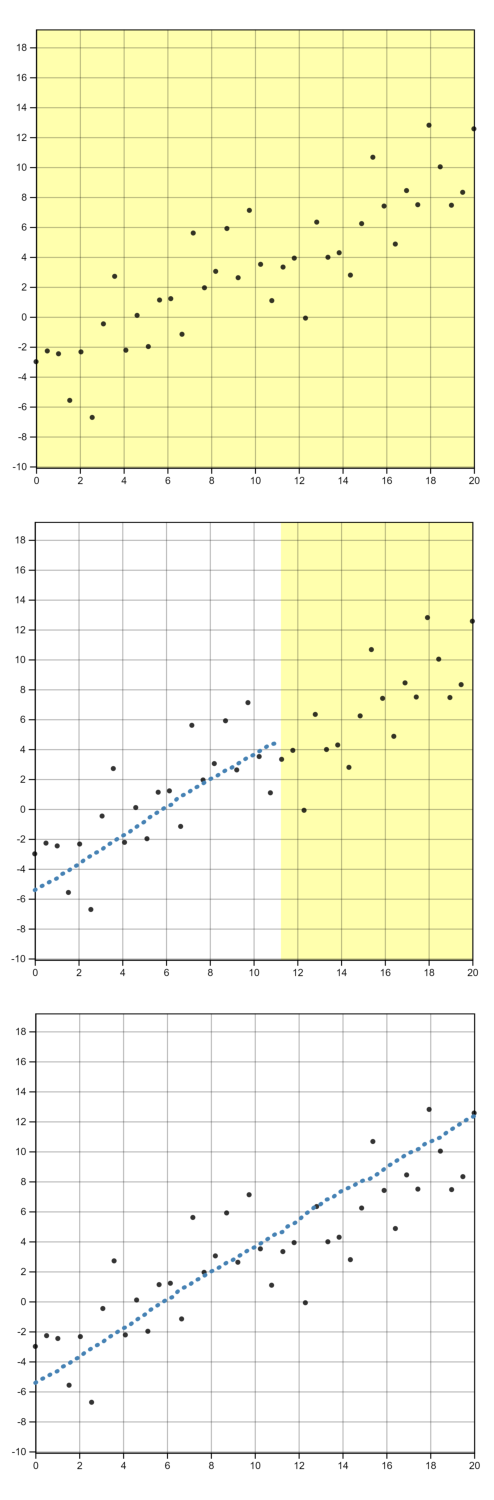
\includegraphics[width=0.7\textwidth,height=\textheight]{./images/fig-you-draw-it-task-plot-1.pdf}
\DIFaddendFL 

}

\caption{\label{fig-you-draw-it-task-plot}You Draw It task plot as shown
to user. \DIFdelbeginFL %DIFDELCMD < \\
%DIFDELCMD < %%%
\textbf{\DIFdelFL{left:}} %DIFAUXCMD
\DIFdelendFL \DIFaddbeginFL \textbf{\DIFaddFL{top:}} \DIFaddendFL Initial state, with instructions\DIFdelbeginFL \emph{\DIFdelFL{Use your mouse to
fill in the trend in the yellow box region.}}%DIFAUXCMD
%DIFDELCMD < \\
%DIFDELCMD < %%%
\DIFdelendFL \DIFaddbeginFL \DIFaddFL{,
}\textit{\DIFaddFL{Use your mouse to fill in the trend in the yellow box region.}}
\DIFaddendFL \textbf{middle:} User view during task completion. \DIFdelbeginFL %DIFDELCMD < \\
%DIFDELCMD < %%%
\textbf{\DIFdelFL{right:}} %DIFAUXCMD
\DIFdelendFL \DIFaddbeginFL \textbf{\DIFaddFL{bottom:}}
\DIFaddendFL Finished state\DIFaddbeginFL \DIFaddFL{.}\DIFaddendFL }

\end{figure}

As shown in Figure~\ref{fig-you-draw-it-task-plot}, the user-filled
portion of the plot is represented with a yellow rectangle, which adapts
to the user's input and spans any missing values. When the box
disappears, the array is filled in and the user can submit their
response.

One challenge introduced by adding this visual cue is that D3 uses
Scalable Vector Graphics (SVG) to render elements. Adding an additional
layer meant that we had to ensure that not only the grids, lines, and
points of the default scatterplot and trend line rendered in the correct
order, but that the yellow box rendered behind all of these points as
well so that no information was masked; and that this layer order
updated in real time.

\hypertarget{connecting-to-shiny}{%
\subsection{Connecting to Shiny}\label{connecting-to-shiny}}

Shiny Messages are used to communicate the user interaction between the
JavaScript code and the R environment. The initial plot is rendered
using Shiny's \texttt{RenderD3} and \texttt{d3Output} functions;
subsequent user interactions are controlled via the JavaScript code.
Once the user is finished modifying the plot, they can submit their
response, so long as they have filled in all of the points. This is
enforced using Shiny's message-passing interface and a JavaScript hook
that notifies Shiny when the array of user-drawn points is completely
filled in. Once the user is done drawing the line, we save the results
of the drawn line to a SQLite database, using Shiny to pass data from
JavaScript to R. The connections between each portion of the app are
shown in Figure~\ref{fig-you-draw-it-code-sketch}.

\begin{figure}

{\centering \DIFdelbeginFL %DIFDELCMD < \includegraphics{images/code-sketch-2.png}
%DIFDELCMD < %%%
\DIFdelendFL \DIFaddbeginFL 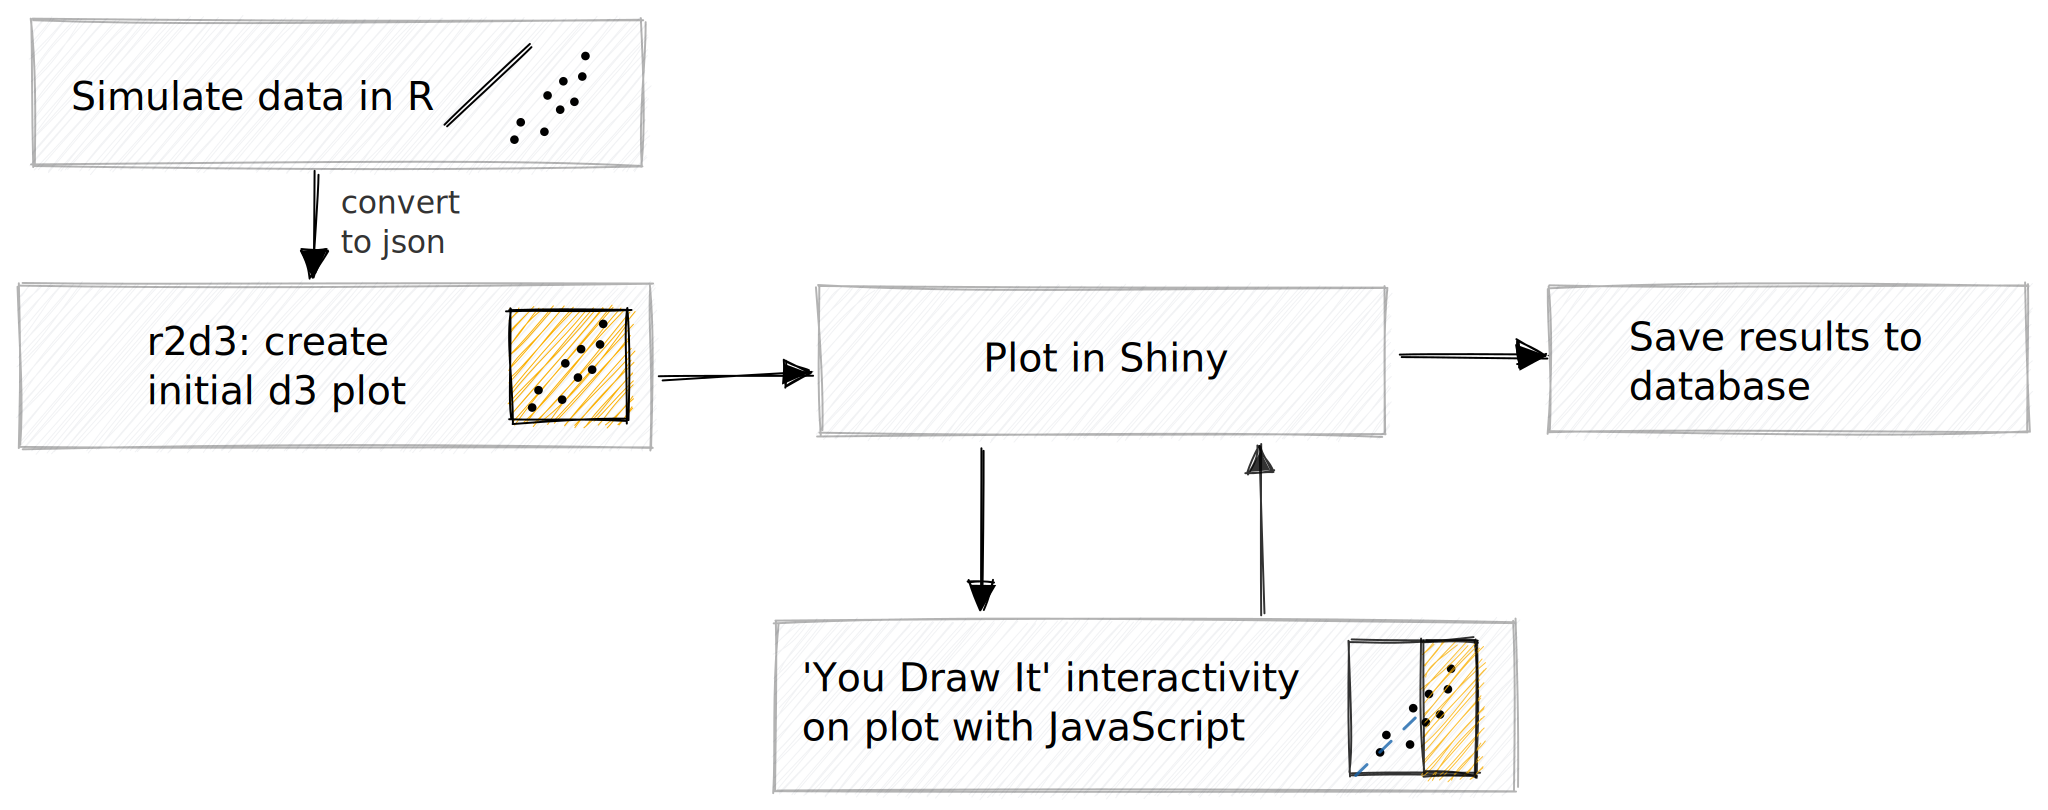
\includegraphics{images/code-sketch.png}
\DIFaddendFL 

}

\caption{\label{fig-you-draw-it-code-sketch}Sketch of underlying code
for `You Draw It', illustrating the data simulation conducted in R, the
initial setup of the visual stimuli with D3 source code, along with the
iterative process between the user interaction and plotting in Shiny.
Once the user is done drawing the line, we saved the results of the
drawn line to a database for analysis.}

\end{figure}

One additional challenge when integrating the D3 graphics into the Shiny
application is that by default, most Shiny applications use a reactive
framework that adjusts to the user's browser size. When working with D3,
however, this can be problematic: most D3 parameters are specified at
the pixel level. The discontinuity between the assumptions of Shiny and
D3 meant that we had to fix the size of the Shiny element, and then
perform a check to ensure that the user's screen was sufficiently big to
render the plot. While in an ideal world, users could participate using
cell phones, tablets, and traditional laptop/desktop computers,
functionally our checks limited users' ability to participate using
smaller screen sizes found in cell phones and some tablets.
Additionally, after some feedback by laptop users during pilot testing,
we included an additional requirement that participants have a computer
mouse available; the results from touchpad users were qualitatively
different (more jagged) in ways suggesting that the recorded data did
not adequately describe users' perceptions.

\hypertarget{application}{%
\section{Application}\label{application}}

\hypertarget{validation-study}{%
\subsection{Validation Study}\label{validation-study}}

We conducted a study in order to validate `You Draw It' as a method for
graphical testing, comparing results to the less technological method
utilized in Mosteller et al. (1981). The original study asked 153
graduate students and postdoctoral researchers in an Introductory
Biostatistics course to fit lines by eye to a set of four points (S, F,
V, N), each set with differing slope and variance properties, using an
8.5 x 11 inch transparency with a straight line etched across the
middle. Researchers conducted the study with a latin square experimental
design to test for a practice effect on the task. Qualitative analysis
suggested that participants tended to fit the slope of the first
principal component (minimizes Euclidean distance) as opposed to the
slope from the ordinary least squares regression (minimizes vertical
distance) Figure~\ref{fig-pca-plot} and found no effect of order.

\begin{figure}

{\centering \includegraphics[width=0.7\textwidth,height=\textheight]{./images/fig-pca-plot-1.pdf}

}

\caption{\label{fig-pca-plot}Comparison between an OLS regression
equation which minimizes the vertical distance of points from the line
and a regression equation with a slope calculated by the first principal
component which minimizes the smallest distance of points from the
line.}

\end{figure}

In our study, we replicated Mosteller et al. (1981) using the `You Draw
It' method and simulated data with parameter coefficients selected to
reflect those from the four data sets in the original study. Data were
simulated based on a linear model with additive errors: \begin{align}
y_i & = \beta_0 + \beta_1 x_i + e_i \\
\text{with } e_i & \sim N(0, \sigma^2). \nonumber
\end{align} For each participant, four unique data sets were randomly
and independently generated from the underlying parameters at the
beginning of the study and mapped to a scatterplot graphic. When
participants started the study, they were first asked to complete two
practice plots - accompanied by instructions and a .gif demonstrating
the task - in order to train them in the skills associated with
executing the task. The four `You Draw It' task plots associated with
the selected parameters followed the practice plots in a random order
for each individual; these plots were interspersed with plots from a
different experiment.

Participants were recruited via Prolific\DIFaddbegin \DIFadd{, a crowd sourcing platform for
researchers to recruit participants for their online studies, }\DIFaddend in March
2022; while this study does utilize a convenience sample, as this is
primarily a perceptual task, previous results have found few differences
between expert and non-expert participants in this context (VanderPlas
and Hofmann 2015). The study was conducted and distributed via a Shiny
application and participants completed the tasks on their own computer,
with a computer mouse, and in an environment of their choosing. The data
from this study were collected to validate this method of graphical
testing, with the hopes of providing a new tool to assess graphical
perception interactively.

\hypertarget{data-analysis-and-results}{%
\subsection{Data Analysis and Results}\label{data-analysis-and-results}}

As a part of the validation study, we collected data for each
participant drawn trend line, allowing us to conduct formal analyses
which compared the intuitive visually fit lines to statistical
regression results - the original study lacked these formal comparisons,
providing only summaries of averages, variances, and actual (least
squares) values for the slope and intercept of each data set. The
feedback data, stored in a SQLite database, contained the simulated data
points\} - \((x_{ijk}, y_{ijk})\) -, the predicted values from the
statistical regression models - \(\hat y_{ijk,OLS}\), and
\(\hat y_{ijk,PCA}\) -, and the predicted values from the user drawn
line - \(y_{ijk,drawn}\) for parameter choice \(i = 1,2,3,4\),
\(j = 1,...,N_\text{participant}\), and \(x_{ijk}\) value
\(k = 1, ...,4 x_{max} + 1\). Figure~\ref{fig-eyefitting-plots} displays
an example of all three fitted trend lines for parameter choice F.

A unique data set was simulated independently for each participant,
therefore, comparisons of vertical residuals between the user drawn line
and the OLS fitted values
(\(e_{ijk,OLS} = y_{ijk,drawn} - \hat y_{ijk,OLS}\)) and PCA fitted
values (\(e_{ijk,PCA} = y_{ijk,drawn} - \hat y_{ijk,PCA}\)) were used to
assess the accuracy of participant drawn lines. We use mixed model
methods to analyze residual trends and capture the variability due to
participant differences.

\begin{figure}

{\centering \includegraphics{./images/fig-eyefitting-plots-1.pdf}

}

\caption{\label{fig-eyefitting-plots}Visual analysis results for
parameter choice set F. \linebreak \textbf{A.} Example of validation
feedback data where three trend lines show the the OLS fitted, PCA
fitted, and participant drawn values overlaid on the simulated data
points. \linebreak \textbf{B \& C.} Estimated trends of residuals
(vertical deviation of participant drawn points from both the OLS (blue)
and PCA (orange) fitted points) as fit by the (B) linear mixed model and
(C) generalized additive mixed model. A random sample of 75 participants
was selected to display the individual participant residuals behind the
overall trend.}

\end{figure}

We first fit a linear mixed model (LMM) to the OLS and PCA residuals
separately using the \texttt{lmer} function in the \texttt{lme4} package
(Bates et al. 2015), constraining the fit to a linear trend. Parameter
choice, \(x\), and the interaction between \(x\) and parameter choice
were treated as fixed effects with a random participant effect
accounting for variation due to participant. The LMM equation for each
fit (OLS and PCA) residuals is given by: \begin{equation}
y_{ijk,drawn} - \hat y_{ijk,fit} = e_{ijk,fit} = \left[\gamma_0 + \alpha_i\right] + \left[\gamma_{1} x_{ijk} + \gamma_{2i} x_{ijk}\right] + p_{j} + \epsilon_{ijk}
\end{equation} \noindent where

\begin{itemize}
\tightlist
\item
  \(y_{ijk,drawn}\) is the drawn y-value for the \(i^{th}\) parameter
  choice, \(j^{th}\) participant, and \(k^{th}\) increment of
  \(x\)-value
\item
  \(\hat y_{ijk,fit}\) is the fitted y-value for the \(i^{th}\)
  parameter choice, \(j^{th}\) participant, and \(k^{th}\) increment of
  \(x\)-value corresponding to either the OLS or PCA fit
\item
  \(e_{ijk,fit}\) is the residual between the drawn and fitted y-values
  for the \(i^{th}\) parameter choice, \(j^{th}\) participant, and
  \(k^{th}\) increment of \(x\)-value corresponding to either the OLS or
  PCA fit
\item
  \(\gamma_0\) is the overall intercept
\item
  \(\alpha_i\) is the effect of the \(i^{th}\) parameter choice (F, S,
  V, N) on the intercept
\item
  \(\gamma_1\) is the overall slope for \(x\)
\item
  \(\gamma_{2i}\) is the effect of the parameter choice on the slope
\item
  \(x_{ijk}\) is the \(x\)-value for the \(i^{th}\) parameter choice,
  \(j^{th}\) participant, and \(k^{th}\) increment
\item
  \(p_{j} \sim N(0, \sigma^2_\text{participant})\) is the random error
  due to the \(j^{th}\) participant's characteristics
\item
  \(\epsilon_{ijk} \sim N(0, \sigma^2)\) is the residual error.
\end{itemize}

Eliminating the linear trend constraint, we can extend the method and
analysis beyond ordinary least squares by using generalized additive
mixed models (GAMM) to estimate smoothing splines and allow for a more
flexible residual trend. The \texttt{bam} function in the \texttt{mgcv}
(Wood 2017) package was used to fit a GAMM separately to the OLS and
PCA. Parameter choice was treated as a fixed effect with no estimated
intercept and a separate smoothing spline for \(x\) was estimated for
each parameter choice. A random participant effect accounting for
variation due to participant and a random spline for each participant
accounted for variation in spline for each participant. The GAMM
equation for each fit (OLS and PCA) residuals is given by:
\begin{equation}
y_{ijk, drawn} - \hat y_{ijk, fit} = e_{ijk,fit} = \alpha_i + s_{i}(x_{ijk}) + p_{j} + s_{j}(x_{ijk})
\end{equation} \noindent where

\begin{itemize}
\tightlist
\item
  \(y_{ijk,drawn}\) is the drawn y-value for the \(i^{th}\) parameter
  choice, \(j^{th}\) participant, and \(k^{th}\) increment of
  \(x\)-value
\item
  \(\hat y_{ijk,fit}\) is the fitted y-value for the \(i^{th}\)
  parameter choice, \(j^{th}\) participant, and \(k^{th}\) increment of
  \(x\)-value corresponding to either the OLS or PCA fit
\item
  \(e_{ijk,fit}\) is the residual between the drawn and fitted y-values
  for the \(i^{th}\) parameter choice, \(j^{th}\) participant, and
  \(k^{th}\) increment of \(x\)-value corresponding to either the OLS or
  PCA fit
\item
  \(\alpha_i\) is the intercept for the parameter choice \(i\)
\item
  \(s_{i}\) is the smoothing spline for the \(i^{th}\) parameter choice
\item
  \(x_{ijk}\) is the \(x\)-value for the \(i^{th}\) parameter choice,
  \(j^{th}\) participant, and \(k^{th}\) increment
\item
  \(p_{j} \sim N(0, \sigma^2_\text{participant})\) is the error due to
  participant variation
\item
  \(s_{j}\) is the random smoothing spline for each participant.
\end{itemize}

This method allows us to quantitatively compare participant lines to the
OLS and principal component regression lines, which is an improvement
over the qualitative approach in Mosteller et al. (1981). While the
statistical models were fit to all four parameter choices,
Figure~\ref{fig-eyefitting-plots} displays the estimated trends of
residuals (vertical deviation of participant drawn points from both the
OLS and PCA fitted points) as modeled by a LMM and GAMM respectively for
parameter choice set F. A random sample of 75 participants was selected
to display individual participant residuals behind the overall residual
trend. Examining the plots, the estimated trends of PCA residuals
(orange) appear to align more parallel and closer to the \(y=0\)
horizontal (dashed) line than the OLS residuals (blue). In particular,
this trend was more prominent in parameter choices with large variances.
Results from our study were consistent with those found in the original
study; when shown points following a linear trend, participants tended
to fit the slope of the first principal component Our study established
`You Draw It' as a method for graphical testing and reinforced the
differences between intuitive visual model fitting and statistical model
fitting, providing information about human perception as it relates to
the use of statistical graphics.

\hypertarget{extension-to-non-linear-data}{%
\subsection{Extension to Non-linear
Data}\label{extension-to-non-linear-data}}

The analysis method presented above extends nicely beyond the linear
regressions tested in Mosteller et al. (1981). Here we briefly
demonstrate this with an example from a study examining participants
ability to make forecasts for exponentially increasing data on log and
linear scales. Along with analyzing the feedback data with the GAMM
method for flexibility due to non-linear data, we used spaghetti plots
to conduct a visual analysis of participant forecasts compared to the
non-linear least squares statistical model and make comparisons between
two chart design features Figure~\ref{fig-exponential-spaghetti-plot}.
The combination of the GAMM analysis and visual display demonstrates the
strength of the `You Draw It' method for testing statistical graphics.

\begin{figure}

{\centering \includegraphics{./images/fig-exponential-spaghetti-plot-1.pdf}

}

\caption{\label{fig-exponential-spaghetti-plot}Spaghetti plot of results
from a study which asked participants to forecast trends of
exponentially increasing data. Participants drawn lines on the linear
scale are shown in blue and the log scale are shown in orange.
Variability in the statistically fitted regression lines occurred due to
a unique data set being simulated for each individual; the gray band
shows the range fitted values from the statistically fitted regression
lines.}

\end{figure}

\DIFaddbegin \hypertarget{discussion}{%
\section{Discussion}\label{discussion}}

\DIFadd{The `You Draw It' graphical task presented in this work is an example of
an interactive graphic. Here we discuss the use of `You Draw It' as a tool for
interactive reading, interactive testing, and interactive teaching as a
way to increase user experience and user engagement with data. The New
York Times first introduced the `You Draw It' feature as a tool for
interactive reading. The inclusion of interactive graphics in news and
media have been used to inform readers in efforts to reduce
misconceptions and aid in storytelling (Geidner et al. 2015;
George-Palilonis and Spillman 2011, 2013). In our work, we demonstrated
the use of the `You Draw It' method as a tool for interactive testing of
graphics. We collected and compared data from user drawn lines to
statistical results in order to understand perceptual biases. While this
work has many possible directions for future work, there is a strong
application to extend the `You Draw It' tool for interactive teaching.
The line of best fit is introduced in secondary schools as a student's
first encounter with the concept of statistical association between
multiple variables (Casey and Nagle 2016). Casey (2015) and Casey (2016)
conducted task based interviews to examine student's conceptions of the
line of best fit prior to introducing the topic. The implications of
using interactive teaching tools for the line of best fit can help
students make connections between the shift in slope and the location of
the best fit line (Nagle, Casey, and Moore-Russo 2017). Casey and
Wasserman (2015) conducted similar task based interviews with
pre-service mathematics teachers in order to understand the effects
regarding teacher preparation for the teaching of this topic. This
demonstrates the use of the `You Draw It' interactive tool for training
purposes both within a classroom setting and for those in the workforce.
}

\DIFaddend \hypertarget{conclusion}{%
\section{Conclusion}\label{conclusion}}

The data presented in this paper are part of a much broader experiment
on the perception of log scales; while this paper focuses primarily on
the computational implementation of the `You Draw It' method and its
adaptation to testing graphics, we are currently finishing the analysis
and description of the broader experiment, which uses this `You Draw It'
method to assess user prediction of exponential trends.

By introducing an interactive method for assessing eye-fit data
summaries, along with an analysis method which allows us to test
competing hypotheses to determine whether user responses are similar to
particular statistical models, we have provided another tool for
experimentally testing statistical charts. In the future, we hope to
create an R package to more easily facilitate these types of user
experiments, making this technique available to other researchers who
may not be willing to tinker with JavaScript directly.

As with any method for testing statistical graphics, there are a host of
additional studies which would be useful to understand how users react
to the `You Draw It' method and what parameters are most important for
the researcher to control. One avenue of future exploration is to
investigate the effect of axis limits on user anchoring. We know that
the perceptual experience is heavily affected by anchoring to e.g.~axis
breaks, and we would expect that a similar anchoring effect might be
present based on the limits of the plot and the amount of space in \(x\)
and \(y\) provided for the user to draw.

\hypertarget{supplementary-material}{%
\section*{Supplementary Material}\label{supplementary-material}}
\addcontentsline{toc}{section}{Supplementary Material}

\begin{itemize}
\tightlist
\item
  \textbf{`You Draw It' Demonstration Applet:} The shiny app used to
  demonstrate the `You Draw It' method can be accessed at
  \href{https://emily-robinson.shinyapps.io/you-draw-it-validation-applet/}{emily-robinson.shinyapps.io/you-draw-it-validation-applet}.
\item
  \textbf{`You Draw It' Script:} The `You Draw It' JavaScript code can
  be accessed at
  \href{https://github.com/earobinson95/presentations/blob/master/can-you-draw-it/www/you-draw-it.js}{github.com/earobinson95/presentations/blob/master/can-you-draw-it/www/you-draw-it.js}.
\item
  \textbf{Study Applet:} The RShiny applet used to conduct the linear
  and non-linear studies can be accessed at
  \href{https://shiny.srvanderplas.com/perception-of-statistical-graphics/}{shiny.srvanderplas.com/perception-of-statistical-graphics/}.
\item
  \textbf{Study Applet Code:} The code used to create the RShiny applet
  for data collection can be found at
  \href{https://github.com/earobinson95/log-perception-prolific/tree/main/perception-of-statistical-graphics}{github.com/earobinson95/log-perception-prolific/tree/main/perception-of-statistical-graphics}.
\item
  \textbf{Participant Data (Linear):} De-identified participant data
  collected in the linear study and used for analyses are available to
  be downloaded from GitHub at
  \href{https://github.com/earobinson95/sdss-2022-you-draw-it-manuscript/raw/master/data/eyefitting-model-data.csv}{github.com/earobinson95/sdss-2022-you-draw-it-manuscript/raw/master/data/eyefitting-model-data.csv}.
\item
  \textbf{Participant Data (Non-linear):} De-identified participant data
  collected in the non-linear study and used for analyses are available
  to be downloaded from GitHub at
  \href{https://github.com/earobinson95/sdss-2022-you-draw-it-manuscript/raw/master/data/youdrawit-model-data.csv}{github.com/earobinson95/sdss-2022-you-draw-it-manuscript/raw/master/data/youdrawit-model-data.csv}.
\item
  \textbf{Data Analysis Code:} The code used to replicate the linear and
  non-linear study analysis in this paper can be found at
  \href{https://earobinson95.github.io/sdss-2022-you-draw-it-manuscript/analysis/data-analysis.html}{earobinson95.github.io/sdss-2022-you-draw-it-manuscript/analysis/data-analysis.htmll}.
\end{itemize}

\hypertarget{references}{%
\section*{References}\label{references}}
\addcontentsline{toc}{section}{References}

\hypertarget{refs}{}
\begin{CSLReferences}{1}{0}
\leavevmode\vadjust pre{\hypertarget{ref-aisch2015you}{}}%
Aisch, Gregor, Amanda Cox, and Kevin Quealy. 2015. {``You Draw It: How
Family Income Predicts Children's College Chances.''} \emph{The New York
Times} 28.

\leavevmode\vadjust pre{\hypertarget{ref-lme4-pkg}{}}%
Bates, Douglas, Martin Mächler, Ben Bolker, and Steve Walker. 2015.
{``Fitting Linear Mixed-Effects Models Using {lme4}.''} \emph{Journal of
Statistical Software} 67 (1): 1--48.
\url{https://doi.org/10.18637/jss.v067.i01}.

\leavevmode\vadjust pre{\DIFaddbegin \hypertarget{ref-becker1987dynamic}{}}%DIF > 
\DIFadd{Becker, Richard A, William S Cleveland, and Allan R Wilks. 1987.
}{\DIFadd{``Dynamic Graphics for Data Analysis.''}} \emph{\DIFadd{Statistical Science}} \DIFadd{2
(4): 355--83.
}

\leavevmode\vadjust \DIFadd{pre}{\DIFaddend \hypertarget{ref-bostock2011d3}{}}%
Bostock, Michael, Vadim Ogievetsky, and Jeffrey Heer. 2011. {``D\(^3\)
Data-Driven Documents.''} \emph{IEEE Transactions on Visualization and
Computer Graphics} 17 (12): 2301--9.

\leavevmode\vadjust pre{\DIFaddbegin \hypertarget{ref-casey2015examining}{}}%DIF > 
\DIFadd{Casey, Stephanie A. 2015. }{\DIFadd{``Examining Student Conceptions of
Covariation: A Focus on the Line of Best Fit.''}} \emph{\DIFadd{Journal of
Statistics Education}} \DIFadd{23 (1).
}

\leavevmode\vadjust \DIFadd{pre}{\hypertarget{ref-casey2016finding}{}}%DIF > 
\DIFadd{---------. 2016. }{\DIFadd{``Finding What Fits.''}} \emph{\DIFadd{Mathematics Teaching in
the Middle School}} \DIFadd{21 (8): 484--91.
}

\leavevmode\vadjust \DIFadd{pre}{\hypertarget{ref-casey2016students}{}}%DIF > 
\DIFadd{Casey, Stephanie A, and Courtney Nagle. 2016. }{\DIFadd{``Students' Use of Slope
Conceptualizations When Reasoning about the Line of Best Fit.''}}
\emph{\DIFadd{Educational Studies in Mathematics}} \DIFadd{92 (2): 163--77.
}

\leavevmode\vadjust \DIFadd{pre}{\hypertarget{ref-casey2015teachers}{}}%DIF > 
\DIFadd{Casey, Stephanie A, and Nicholas H Wasserman. 2015.
}{\DIFadd{``TEACHERS'KNOWLEDGE ABOUT INFORMAL LINE OF BEST FIT.''}}
\emph{\DIFadd{Statistics Education Research Journal}} \DIFadd{14 (1): 8--35.
}

\leavevmode\vadjust \DIFadd{pre}{\DIFaddend \hypertarget{ref-ciccione2021can}{}}%
Ciccione, Lorenzo, and Stanislas Dehaene. 2021. {``Can Humans Perform
Mental Regression on a Graph? Accuracy and Bias in the Perception of
Scatterplots.''} \emph{Cognitive Psychology} 128: 101406.

\leavevmode\vadjust pre{\hypertarget{ref-deming1943statistical}{}}%
Deming, William Edwards. 1943. {``Statistical Adjustment of Data.''}

\leavevmode\vadjust pre{\DIFaddbegin \hypertarget{ref-eick1995high}{}}%DIF > 
\DIFadd{Eick, Stephen G, and Graham J Wills. 1995. }{\DIFadd{``High Interaction
Graphics.''}} \emph{\DIFadd{European Journal of Operational Research}} \DIFadd{81 (3):
445--59.
}

\leavevmode\vadjust \DIFadd{pre}{\DIFaddend \hypertarget{ref-finney1951subjective}{}}%
Finney, DJ. 1951. {``Subjective Judgment in Statistical Analysis: An
Experimental Study.''} \emph{Journal of the Royal Statistical Society:
Series B (Methodological)} 13 (2): 284--97.

\leavevmode\vadjust pre{\hypertarget{ref-furic_2017}{}}%
Furic, Benoit. 2017. {``You-Draw-It-Graph: The User Can Draw His Own
Graph Line and Compare with the Reality.''} \emph{GitHub}.
\url{https://github.com/BenoitFuric/you-draw-it-graph}.

\leavevmode\vadjust pre{\DIFaddbegin \hypertarget{ref-geidner2015role}{}}%DIF > 
\DIFadd{Geidner, Nick, Ivanka Pjesivac, Iveta Imre, Ioana Coman, and Dzmitry
Yuran. 2015. }{\DIFadd{``The Role of Interactive Graphics in Reducing
Misperceptions in the Electorate.''}} \emph{\DIFadd{Visual Communication
Quarterly}} \DIFadd{22 (3): 133--45.
}

\leavevmode\vadjust \DIFadd{pre}{\hypertarget{ref-george2011interactive}{}}%DIF > 
\DIFadd{George-Palilonis, Jennifer, and Mary Spillman. 2011. }{\DIFadd{``Interactive
Graphics Development: A Framework for Studying Innovative Visual Story
Forms.''}} \emph{\DIFadd{Visual Communication Quarterly}} \DIFadd{18 (3): 167--77.
}

\leavevmode\vadjust \DIFadd{pre}{\hypertarget{ref-george2013storytelling}{}}%DIF > 
\DIFadd{---------. 2013. }{\DIFadd{``Storytelling with Interactive Graphics: An Analysis
of Editors' Attitudes and Practices.''}} \emph{\DIFadd{Visual Communication
Quarterly}} \DIFadd{20 (1): 20--27.
}

\leavevmode\vadjust \DIFadd{pre}{\DIFaddend \hypertarget{ref-mosteller1981eye}{}}%
Mosteller, Frederick, Andrew F Siegel, Edward Trapido, and Cleo Youtz.
1981. {``Eye Fitting Straight Lines.''} \emph{The American Statistician}
35 (3): 150--52.

\leavevmode\vadjust pre{\DIFaddbegin \hypertarget{ref-nagle2017slope}{}}%DIF > 
\DIFadd{Nagle, Courtney, Stephanie Casey, and Deborah Moore-Russo. 2017.
}{\DIFadd{``Slope and Line of Best Fit: A Transfer of Knowledge Case Study.''}}
\emph{\DIFadd{School Science and Mathematics}} \DIFadd{117 (1-2): 13--26.
}

\leavevmode\vadjust \DIFadd{pre}{\DIFaddend \hypertarget{ref-pearce_2019}{}}%
Pearce, Adam. 2019. {``You-Draw-It.''} \emph{Observable}.
\url{https://bl.ocks.org/1wheel/07d9040c3422dac16bd5be741433ff1e}.

\leavevmode\vadjust pre{\hypertarget{ref-r-software}{}}%
R Core Team. 2022. \emph{R: A Language and Environment for Statistical
Computing}. Vienna, Austria: R Foundation for Statistical Computing.
\url{https://www.R-project.org/}.

\leavevmode\vadjust pre{\hypertarget{ref-r2d3pkg}{}}%
Strayer, Nick, Javier Luraschi, and JJ Allaire. 2020. \emph{R2d3:
Interface to 'D3' Visualizations}.
\url{https://CRAN.R-project.org/package=r2d3}\DIFaddbegin \DIFadd{.
}

\leavevmode\vadjust \DIFadd{pre}{\hypertarget{ref-unwin1999requirements}{}}%DIF > 
\DIFadd{Unwin, Antony. 1999. }{\DIFadd{``Requirements for Interactive Graphics Software
for Exploratory Data Analysis.''}} \emph{\DIFadd{Computational Statistics}} \DIFadd{14
(1): 7--22}\DIFaddend .

\leavevmode\vadjust pre{\hypertarget{ref-unwin1988eyeballing}{}}%
Unwin, Antony R, and Graham Wills. 1988. {``Eyeballing Time Series.''}
In \emph{Proceedings of the 1988 ASA Statistical Computing Section},
263--68.

\leavevmode\vadjust pre{\hypertarget{ref-usenergyinformationadministrationWeeklyAllGrades2022}{}}%
US Energy Information Administration. 2022. {``Weekly {U}.{S}. {All}
{Grades} {All} {Formulations} {Retail} {Gasoline} {Prices} ({Dollars}
Per {Gallon}).''} \emph{US Energy Information Administration Independent
Statistics \& Analysis}.
\url{https://www.eia.gov/dnav/pet/hist/LeafHandler.ashx?n=PET\&s=EMM_EPM0_PTE_NUS_DPG\&f=W}.

\leavevmode\vadjust pre{\hypertarget{ref-vanderplas2015spatial}{}}%
VanderPlas, Susan, and Heike Hofmann. 2015. {``Spatial Reasoning and
Data Displays.''} \emph{IEEE Transactions on Visualization and Computer
Graphics} 22 (1): 459--68.

\leavevmode\vadjust pre{\hypertarget{ref-wattenberger-fullstack}{}}%
Wattenberger, Amelia. 2019. \emph{Fullstack D3 and Data Visualization:
Build Beautiful Data Visualizations and Dashboards with D3}.
Fullstack.io.

\leavevmode\vadjust pre{\hypertarget{ref-mgcv_pkg}{}}%
Wood, S. N. 2017. \emph{Generalized Additive Models: An Introduction
with r}. 2nd ed. Chapman; Hall/CRC.

\end{CSLReferences}



\end{document}
